\chapter{Appendix}
\label{appendix:main}

This appendix provides supplementary materials for the thesis, including prompt templates, ontology structure, dataset description, execution traces, and web interface documentation.

%======================================================================
% A.1 Prompt Templates
%======================================================================
\section{Prompt Templates}
\label{appendix:prompts}

This section presents the complete prompt templates used in our semantic annotation system. The prompts are designed to guide LLMs in mapping table columns to ontology classes through structured reasoning.

\subsection{System Message}

The system message establishes the LLM's role as a semantic annotation expert:

\begin{lstlisting}[basicstyle=\small\ttfamily, breaklines=true, frame=single, caption={System Message}, label={lst:system-message}]
You are a knowledgeable assistant who helps map tabular
data columns to ontology classes. You have expert knowledge
in semantic table annotation, i.e., table column-to-ontology
class mappings. Your goal is to determine the most
semantically appropriate ontology class (or set of classes)
for a given column, based on the provided table name, table
header, example data, column name, and the ontology classes
at current level.
\end{lstlisting}

\subsection{Human Message Template}

The human message provides the table context and candidate ontology classes:

\begin{lstlisting}[basicstyle=\small\ttfamily, breaklines=true, frame=single, caption={Human Message Template}, label={lst:human-message}]
We have a table named '{table_name}' which has several
columns. Below is the table in Markdown format, including
column headers and a few example rows:

{table_in_markdown}

We are currently focusing on ontology classes at the given
level. Below are {class_description}:
{current_level_ontology_classes}

We want to determine the best fitting ontology class (or
class path if multiple levels are considered) for the
following column: '{column_name}'.

Instructions:
1. Review the column name and the example data.
2. Based on the ontology classes provided, select the most
   suitable ontology class or classes (or ancestor class
   or classes) of the corresponding class that best
   describe the semantic meaning of this column.
3. {output_instruction}

Note: The provided set of ontology classes might not be
complete. If you think none of the given classes are
suitable, you can indicate that accordingly.
\end{lstlisting}

\subsection{Output Instructions}

\subsubsection{Direct Prompt Output}

For direct prompts, the LLM is instructed to provide only the answer:

\begin{lstlisting}[basicstyle=\small\ttfamily, breaklines=true, frame=single, caption={Direct Prompt Output Instruction}, label={lst:direct-output}]
Output the final answer enclosed in <answer></answer> tags,
  3.1 If multiple ontology classes are required to describe
      the column, split the classes with a comma, for
      example, <answer>ontology_class1, ontology_class2,
      ..., ontology_classN</answer>
  3.2 If no suitable class is found, respond with
      <answer>-</answer>.
\end{lstlisting}

\subsubsection{Chain-of-Thought (CoT) Output}

For CoT prompts, the LLM first provides reasoning before the answer:

\begin{lstlisting}[basicstyle=\small\ttfamily, breaklines=true, frame=single, caption={Chain-of-Thought Output Instruction}, label={lst:cot-output}]
First, output your reasoning enclosed in
<reasoning></reasoning> tags. Then output the final answer
enclosed in <answer></answer> tags,
  3.1 If multiple ontology classes are required to describe
      the column, split the classes with a comma, for
      example, <answer>ontology_class1, ontology_class2,
      ..., ontology_classN</answer>
  3.2 If no suitable class is found, respond with
      <answer>-</answer>.
\end{lstlisting}

\subsection{Prompt Variants}

\begin{table}[htbp]
\centering
\caption{Prompt Template Variants}
\label{tab:prompt-variants}
\begin{tabular}{lll}
\toprule
\textbf{Variant} & \textbf{Class Description} & \textbf{Output Type} \\
\midrule
Direct Single & ``the set of the ontology classes'' & Direct \\
Direct EDM & ``a subset of the ontology classes'' & Direct \\
CoT Single & ``the set of the ontology classes'' & CoT \\
CoT EDM & ``a subset of the ontology classes'' & CoT \\
\bottomrule
\end{tabular}
\end{table}


%======================================================================
% A.2 Building Energy Ontology Structure
%======================================================================
\section{Building Energy Ontology Structure}
\label{appendix:beo}

This section describes the Building Energy Ontology (BEO) used in our experiments.

\subsection{Ontology Overview}

\begin{table}[htbp]
\centering
\caption{BEO Ontology Statistics}
\label{tab:beo-stats}
\begin{tabular}{lr}
\toprule
\textbf{Property} & \textbf{Value} \\
\midrule
Ontology Name & Building Energy Ontology (BEO) \\
Version & v0.5.0 \\
Namespace & \texttt{http://www.owl-ontologies.com/beo\#} \\
Total Classes & 602 \\
Maximum Depth & 8 \\
Created & 2024-02-09 \\
Modified & 2024-04-10 \\
Authors & Zhiyu Pan, Lei Zhao \\
\bottomrule
\end{tabular}
\end{table}

\subsection{Top-Level Class Hierarchy}

The BEO ontology organizes concepts into the following major categories under the root class \texttt{owl:Thing}:

\begin{table}[htbp]
\centering
\caption{Major BEO Class Categories}
\label{tab:beo-classes}
\begin{tabular}{ll}
\toprule
\textbf{Category} & \textbf{Description} \\
\midrule
TemporalEntity & Time-related concepts (Interval, Instant) \\
Measurement & Measurement values and units \\
Property & Observable and measurable properties \\
Location & Geographical and spatial concepts \\
District & Administrative and geographical regions \\
Building & Building structures and components \\
Space & Spatial zones and building spaces \\
Device & Sensors, actuators, and meters \\
EnergySystem & Energy production and consumption systems \\
PowerSystemResource & Power delivery and distribution \\
KPI & Key Performance Indicators \\
Observation & Sensor observations and values \\
UnitOfMeasure & Measurement units (Energy, Power, Currency) \\
EntityType & Type classifications \\
SocialUnit & People and organizations \\
\bottomrule
\end{tabular}
\end{table}

\subsection{Selected Class Hierarchies}

\subsubsection{Temporal Classes}
\begin{itemize}
    \item \textbf{TemporalEntity}
    \begin{itemize}
        \item Interval -- A time span with beginning and end
        \item Instant -- A single point in time
    \end{itemize}
\end{itemize}

\subsubsection{Measurement Classes}
\begin{itemize}
    \item \textbf{Measurement}
    \begin{itemize}
        \item EnergyUnit -- Energy measurements (kWh, MWh)
        \item PowerUnit -- Power measurements (W, kW)
        \item Currency -- Monetary values
        \item TemperatureUnit -- Temperature measurements
    \end{itemize}
\end{itemize}

\subsubsection{Property Classes}
\begin{itemize}
    \item \textbf{Property}
    \begin{itemize}
        \item PowerEquipment -- Power-related equipment properties
        \item CO2\_level -- Carbon dioxide measurements
        \item EquipmentParameter -- Device configuration parameters
    \end{itemize}
\end{itemize}


%======================================================================
% A.3 Dataset Description
%======================================================================
\section{Dataset Description}
\label{appendix:dataset}

This section provides details about the evaluation dataset used in our experiments.

\subsection{Dataset Overview}

\begin{table}[htbp]
\centering
\caption{Dataset Statistics}
\label{tab:dataset-stats}
\begin{tabular}{lr}
\toprule
\textbf{Property} & \textbf{Value} \\
\midrule
Total Tables & 47 \\
Total Columns & 431 \\
Data Domain & Building Energy Management \\
Data Sources & Building management systems \\
Geographic Origin & Multiple European countries \\
Time Period & 2017--2024 \\
File Format & CSV \\
\bottomrule
\end{tabular}
\end{table}

\subsection{Sample Tables}

\subsubsection{Table 1: School Building Energy Data}

\begin{table}[htbp]
\centering
\caption{Sample Data from Table 1}
\label{tab:sample-table1}
\begin{tabular}{lrrr}
\toprule
\textbf{Month} & \textbf{Usage [kWh]} & \textbf{Cost (net in PLN)} & \textbf{Cost (gross in PLN)} \\
\midrule
2017-01 & 6561.00 & 5148.17 & 6332.24 \\
2017-02 & 6947.88 & 5092.37 & 6263.63 \\
2017-03 & 7254.04 & 5282.47 & 6497.43 \\
2017-04 & 5594.92 & 4917.50 & 6048.52 \\
2017-05 & 5059.80 & 4808.05 & 5913.91 \\
\bottomrule
\end{tabular}
\end{table}

\subsection{Ground Truth Annotation}

Each column in the dataset is annotated with:
\begin{itemize}
    \item \textbf{Level 1 Class}: The top-level ontology class (direct child of \texttt{Thing})
    \item \textbf{Level 2 Class}: The specific subclass within the hierarchy
    \item \textbf{Alternative Paths}: Some columns may have multiple valid classification paths
\end{itemize}

\begin{table}[htbp]
\centering
\caption{Ground Truth Examples from Table 1}
\label{tab:ground-truth-examples}
\begin{tabular}{llll}
\toprule
\textbf{Column} & \textbf{Level 1} & \textbf{Level 2} & \textbf{Path} \\
\midrule
Month & TemporalEntity & Interval & TemporalEntity / Interval \\
Usage [kWh] & Measurement & EnergyUnit & Measurement / EnergyUnit \\
Cost (net in PLN) & Measurement & Currency & Measurement / Currency \\
Cost (gross in PLN) & Measurement & Currency & Measurement / Currency \\
\bottomrule
\end{tabular}
\end{table}

\subsection{Column Type Distribution}

The dataset covers a diverse range of semantic types commonly found in building energy data:

\begin{itemize}
    \item \textbf{Temporal columns}: Dates, timestamps, time intervals, months
    \item \textbf{Measurement columns}: Energy consumption, power readings, costs
    \item \textbf{Spatial columns}: Building names, locations, zones
    \item \textbf{Device columns}: Sensor IDs, meter readings
    \item \textbf{Categorical columns}: Energy types, building types
\end{itemize}


%======================================================================
% A.4 Sample Execution Traces
%======================================================================
\section{Sample Execution Traces}
\label{appendix:traces}

This section presents example execution traces from our annotation system, demonstrating the LLM reasoning process at each hierarchical level.

\subsection{Successful Annotation Example}

The following example shows the annotation process for the ``Month'' column from Table 1 (School building data).

\subsubsection{Level 0: Root Selection}

\textbf{Input Context:}
\begin{itemize}
    \item Table: School building data
    \item Column: Month
    \item Sample values: 2017-01, 2017-02, 2017-03, ...
    \item Candidates: 87 top-level classes
\end{itemize}

\textbf{LLM Reasoning (CoT):}
\begin{quote}
\textit{``The column `Month' contains values such as `2017-01', `2017-02', etc., which represent specific time intervals (months in a year). The semantic meaning of this column is temporal---it identifies the time period to which the data in each row pertains. Among the provided ontology classes, `TemporalEntity' is the most appropriate, as it is commonly used to represent time-related concepts such as dates, times, durations, and intervals. None of the other classes (e.g., Location, Observation, Measurement) are as directly relevant to representing a time period or interval.''}
\end{quote}

\textbf{Selected Class:} \texttt{TemporalEntity}

\textbf{Metrics:}
\begin{itemize}
    \item Latency: 1,834 ms
    \item Input tokens: 783
    \item Output tokens: 136
\end{itemize}

\subsubsection{Level 1: Subclass Selection}

\textbf{Input Context:}
\begin{itemize}
    \item Parent class: TemporalEntity
    \item Candidates: Interval, Instant
\end{itemize}

\textbf{LLM Reasoning (CoT):}
\begin{quote}
\textit{``The `Month' column contains values such as `2017-01', `2017-02', etc., which represent a specific month in a specific year. This is not a single point in time (Instant), but rather a time interval that spans from the beginning to the end of a particular month. Among the provided ontology classes, `Interval' is the most appropriate, as it represents a duration or span of time, which aligns with the semantics of a calendar month.''}
\end{quote}

\textbf{Selected Class:} \texttt{Interval}

\textbf{Final Path:} \texttt{TemporalEntity / Interval}

\textbf{Ground Truth:} \texttt{TemporalEntity / Interval} \checkmark

\subsubsection{Execution Summary}

\begin{table}[htbp]
\centering
\caption{Execution Trace Summary for ``Month'' Column}
\label{tab:trace-summary}
\begin{tabular}{lllrr}
\toprule
\textbf{Level} & \textbf{Parent} & \textbf{Selected} & \textbf{Latency (ms)} & \textbf{Tokens} \\
\midrule
0 & Thing & TemporalEntity & 1,834 & 919 \\
1 & TemporalEntity & Interval & 1,241 & 656 \\
\midrule
\multicolumn{3}{l}{\textbf{Total}} & 3,075 & 1,575 \\
\bottomrule
\end{tabular}
\end{table}

\subsection{Challenging Annotation Example}

Some columns present challenges due to ambiguous headers or limited sample data.

\subsubsection{Example: Ambiguous Column Header}

\textbf{Column:} ``BTN A'' (from Table 2)

\textbf{Challenge:} The column header ``BTN A'' is an abbreviation that does not clearly indicate the semantic meaning. Without domain knowledge, it is difficult to determine whether this represents power consumption, a sensor reading, or device identifier.

\textbf{Ground Truth:} \texttt{Property / PowerEquipment} and \texttt{Measurement / PowerUnit}

\textbf{Observation:} This case demonstrates the importance of sample data in guiding the LLM's decision. Numeric values with units (e.g., kW) help identify measurement-related semantics.


%======================================================================
% A.5 Web Interface Screenshots
%======================================================================
\section{Web Interface Screenshots}
\label{appendix:webui}

This section presents screenshots of the web-based user interface developed for the semantic annotation system.

\begin{figure}[htbp]
    \centering
    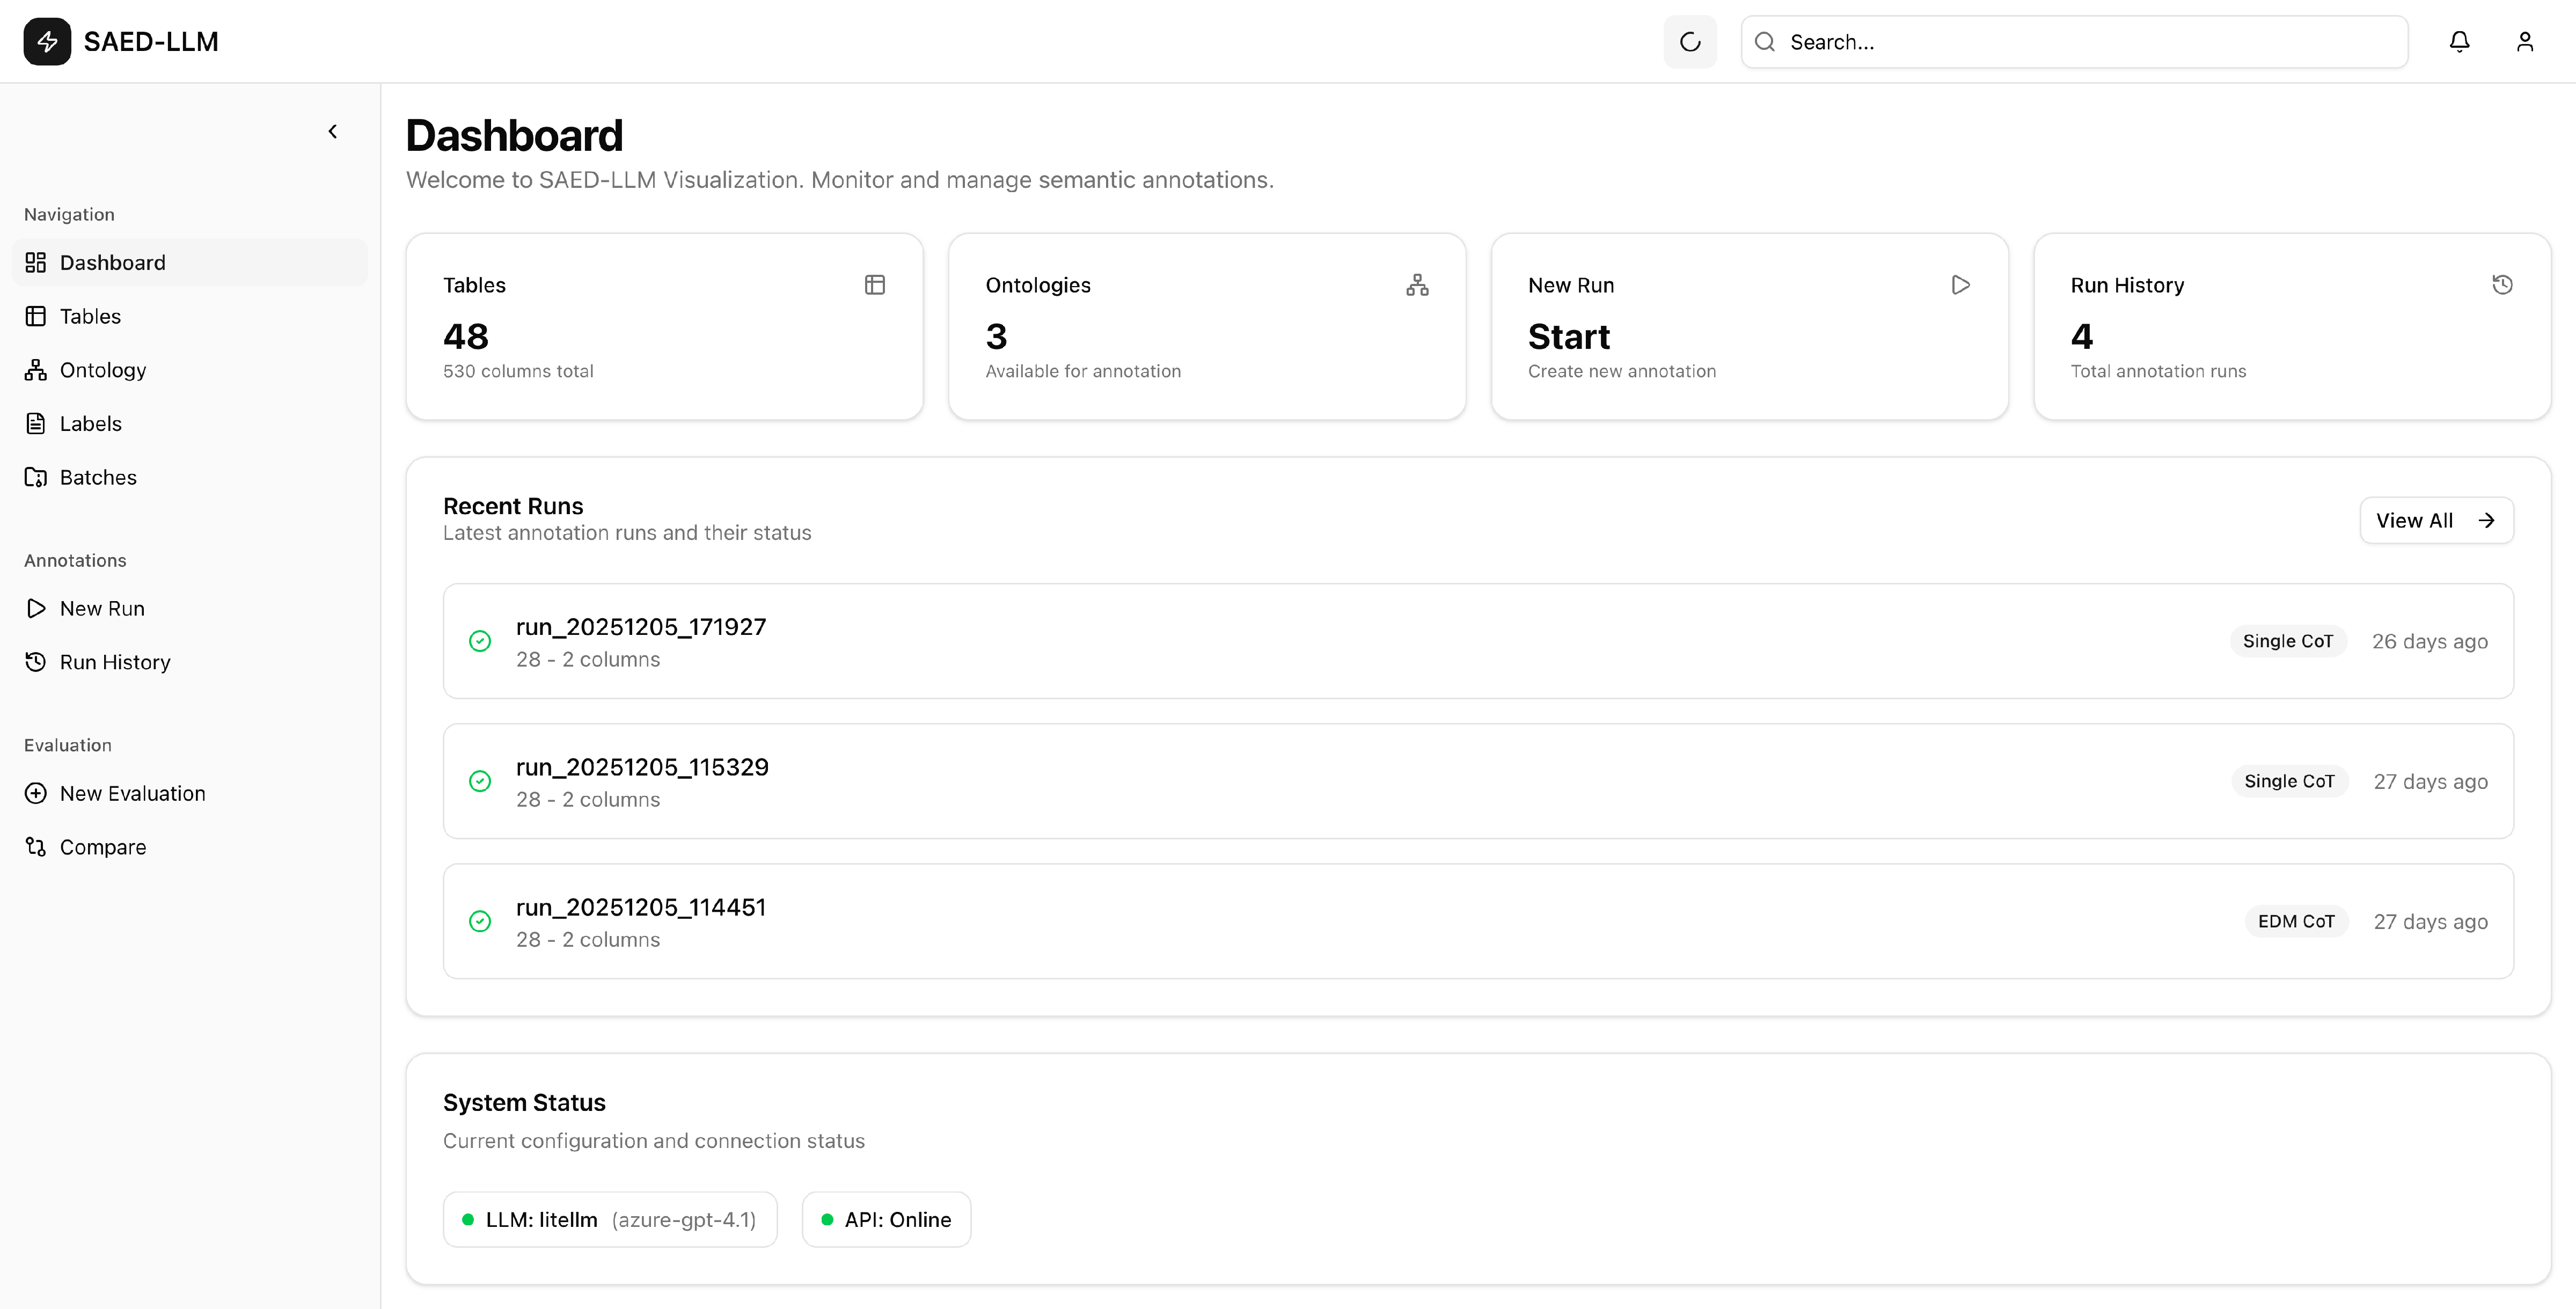
\includegraphics[width=\textwidth]{graphics/canvas/appendix_dashboard.pdf}
    \caption{Dashboard view showing an overview of system status, recent annotation runs, and quick access to main features.}
    \label{fig:webui-dashboard}
\end{figure}

\begin{figure}[htbp]
    \centering
    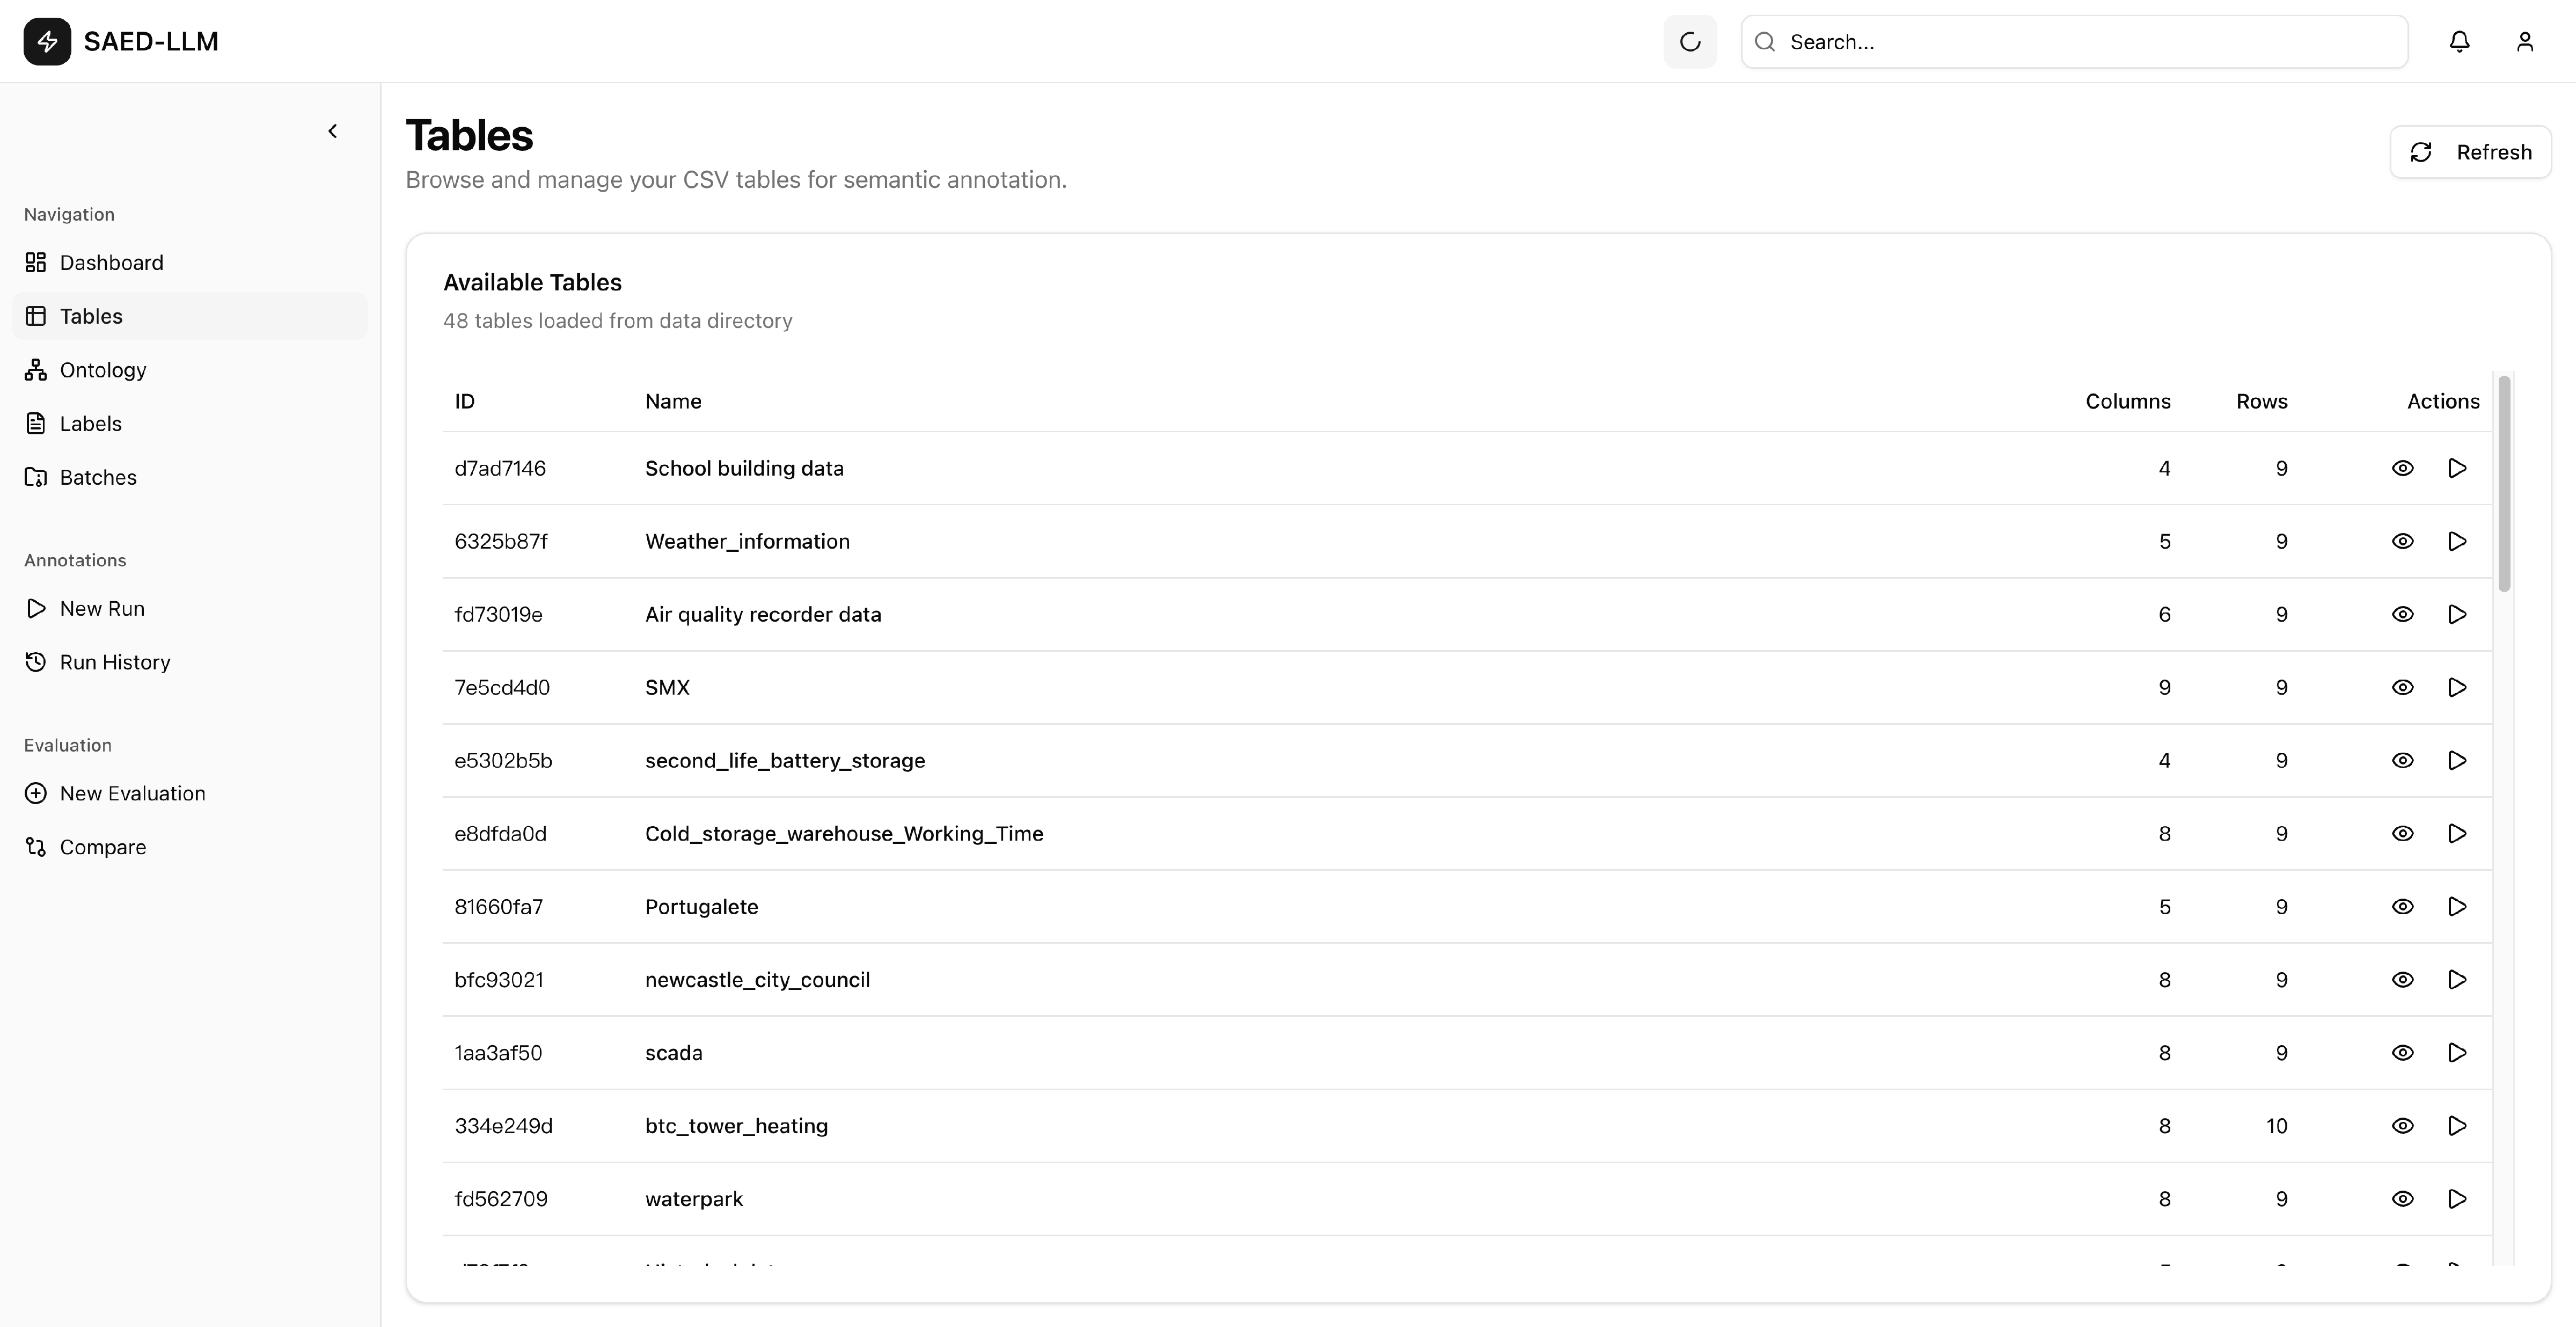
\includegraphics[width=\textwidth]{graphics/canvas/appendix_tables.pdf}
    \caption{Tables management interface for browsing and selecting uploaded CSV files.}
    \label{fig:webui-tables}
\end{figure}

\begin{figure}[htbp]
    \centering
    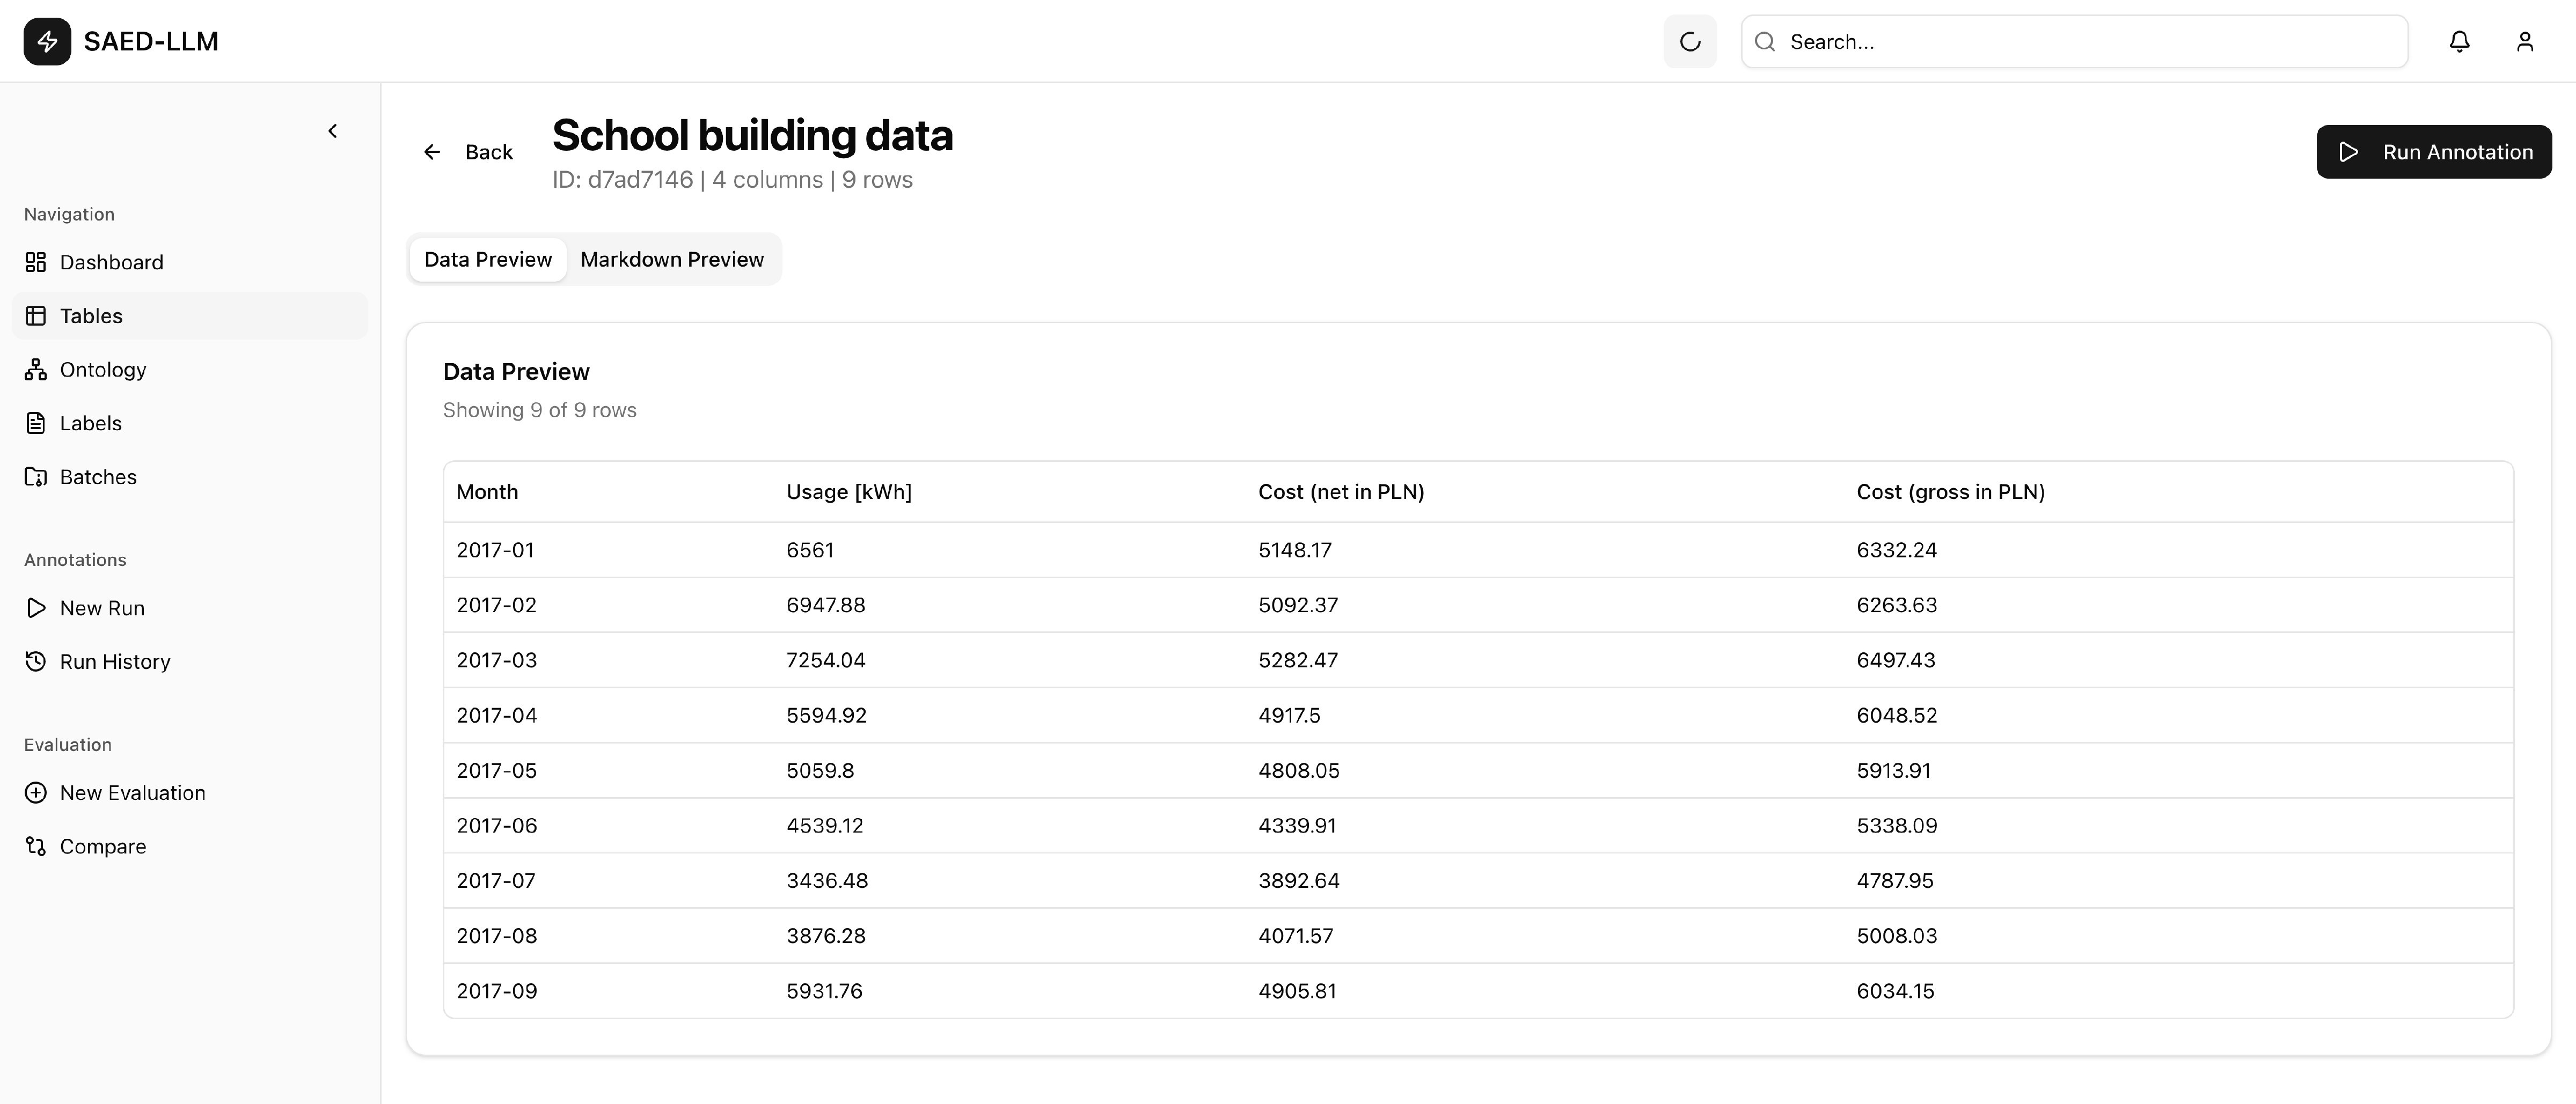
\includegraphics[width=\textwidth]{graphics/canvas/appendix_tables_preview.pdf}
    \caption{Table preview interface displaying column headers and sample data rows.}
    \label{fig:webui-tables-preview}
\end{figure}

\begin{figure}[htbp]
    \centering
    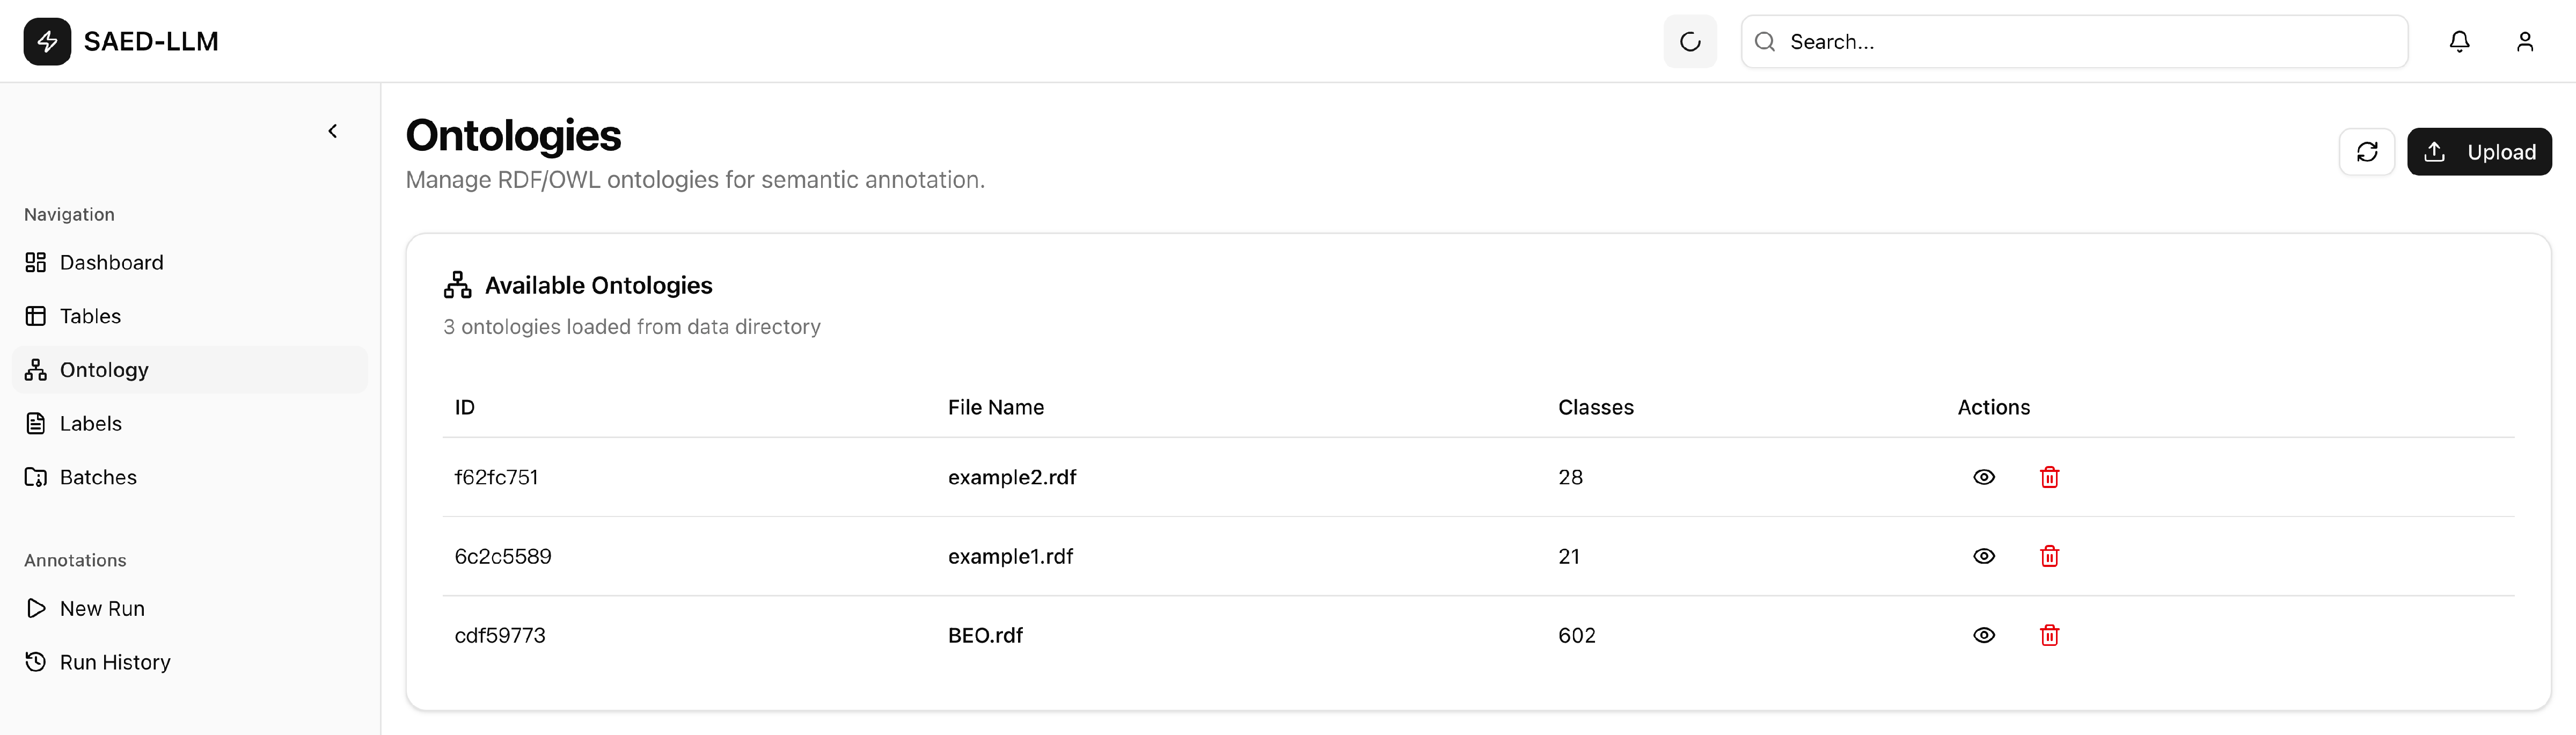
\includegraphics[width=\textwidth]{graphics/canvas/appendix_ontologies.pdf}
    \caption{Ontologies management interface for browsing available ontology files.}
    \label{fig:webui-ontologies}
\end{figure}

\begin{figure}[htbp]
    \centering
    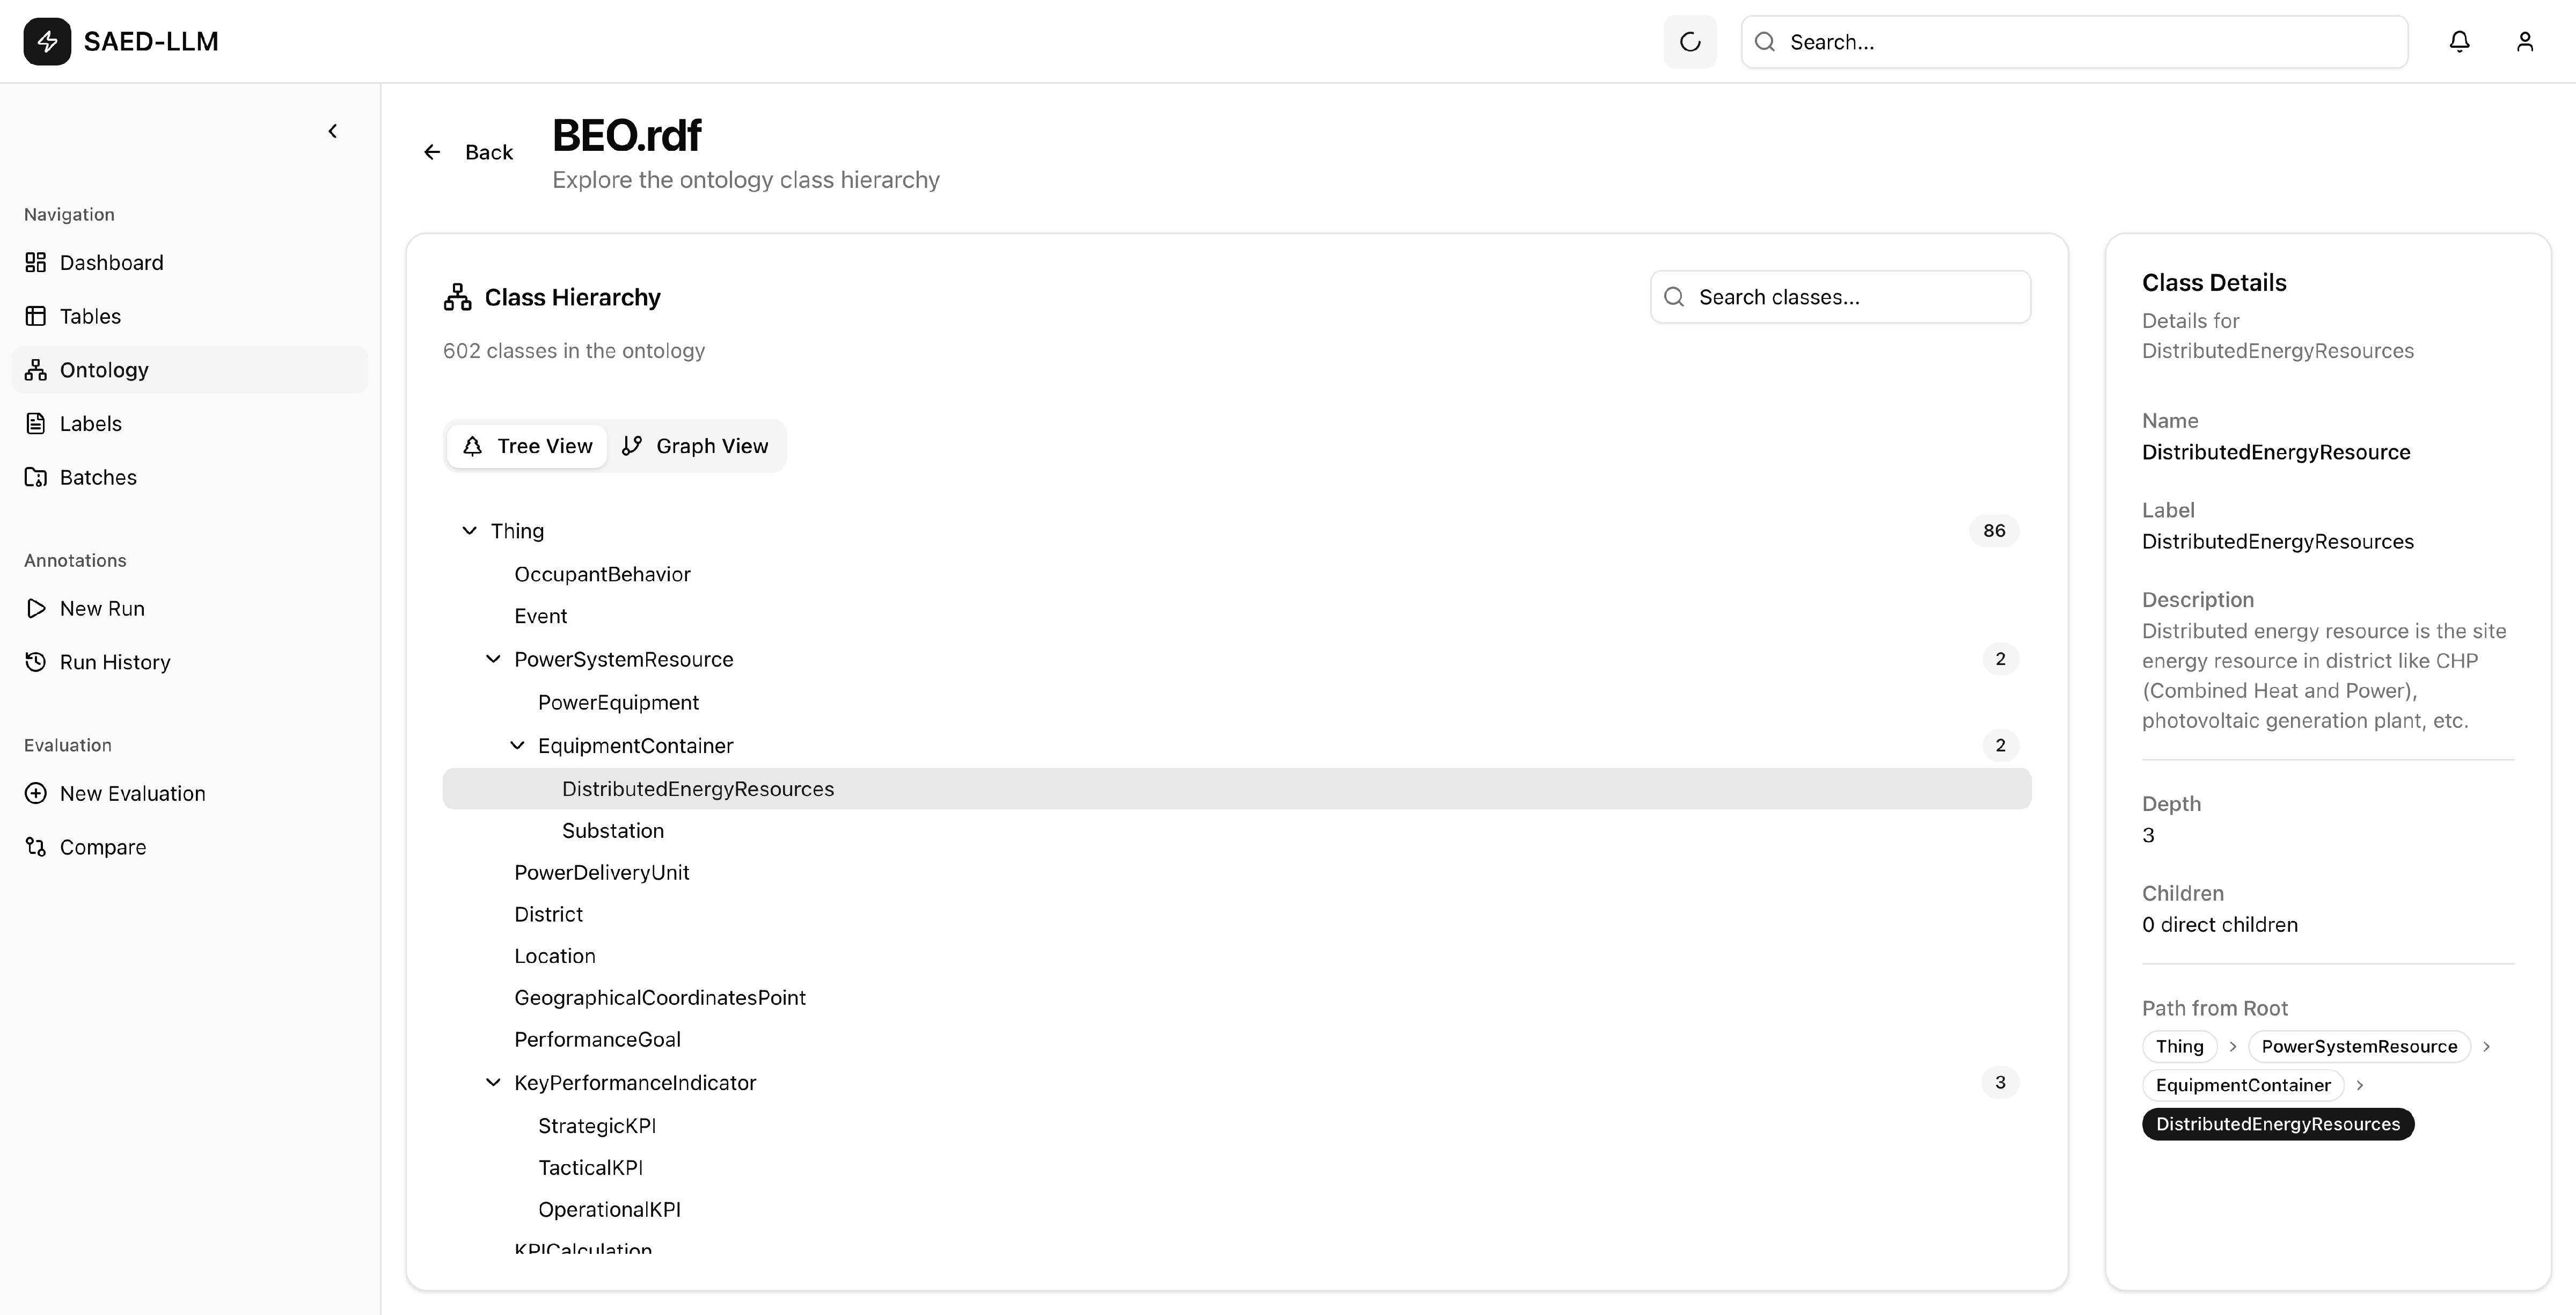
\includegraphics[width=\textwidth]{graphics/canvas/appendix_ontologies_tree_view.pdf}
    \caption{Ontology tree view showing the hierarchical class structure.}
    \label{fig:webui-ontologies-tree}
\end{figure}

\begin{figure}[htbp]
    \centering
    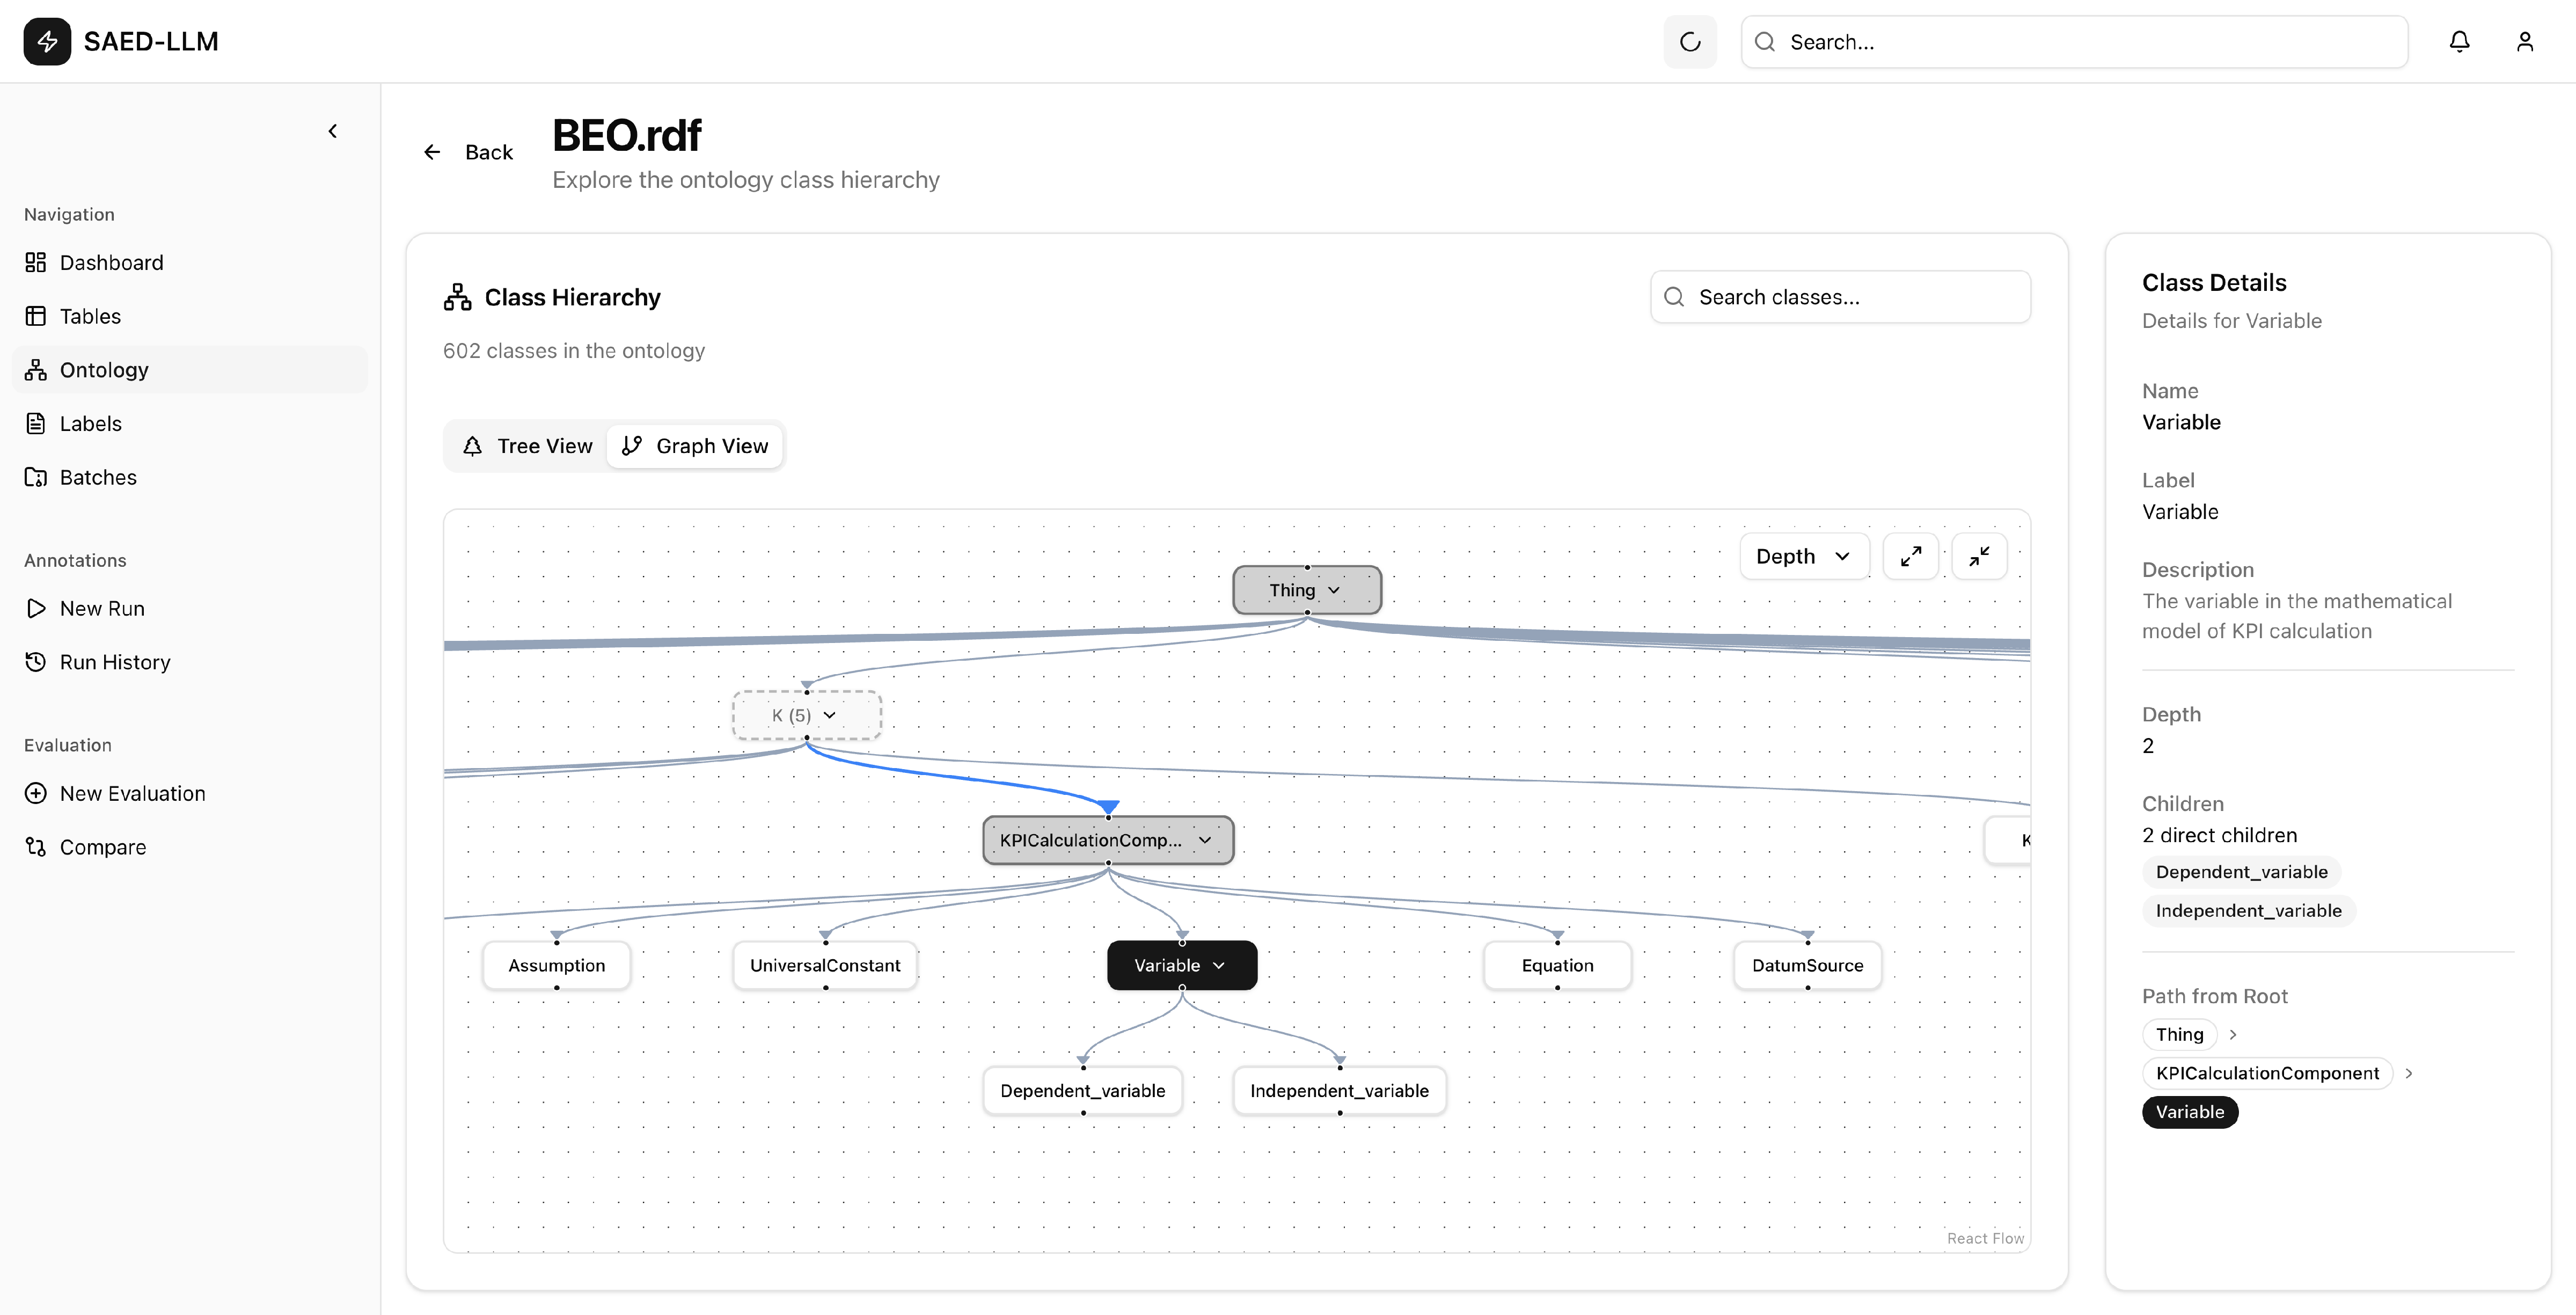
\includegraphics[width=\textwidth]{graphics/canvas/appendix_ontologies_graph_view.pdf}
    \caption{Ontology graph view providing an interactive visualization of class relationships.}
    \label{fig:webui-ontologies-graph}
\end{figure}

\begin{figure}[htbp]
    \centering
    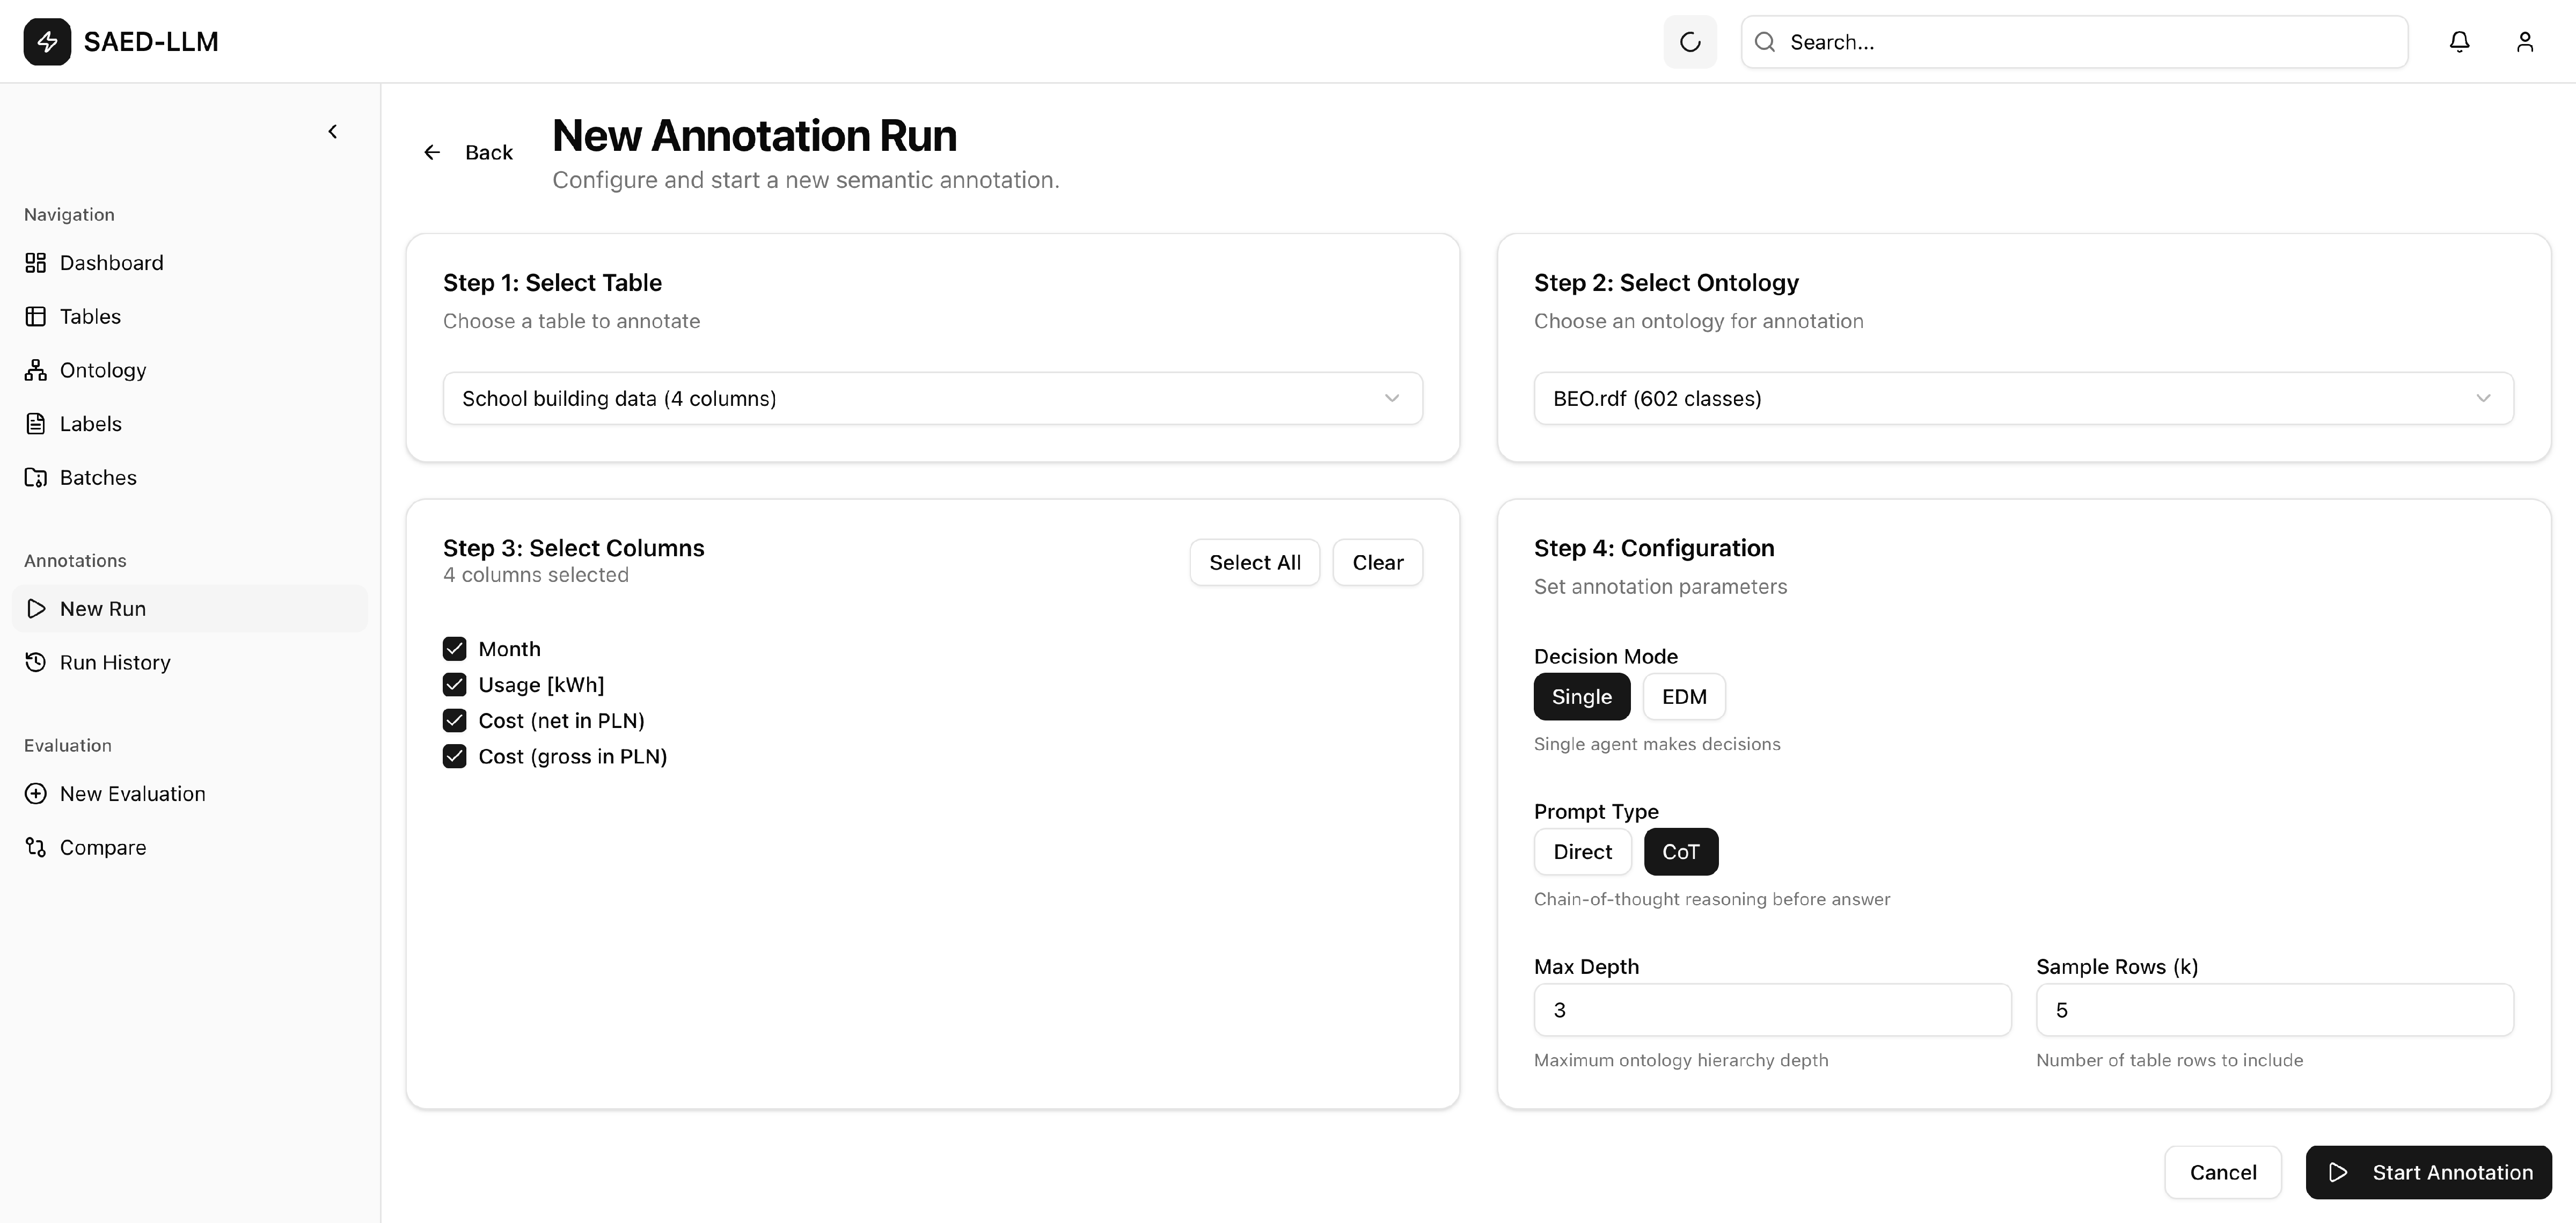
\includegraphics[width=\textwidth]{graphics/canvas/appendix_run.pdf}
    \caption{Annotation run interface showing task configuration and real-time execution progress.}
    \label{fig:webui-run}
\end{figure}

\begin{figure}[htbp]
    \centering
    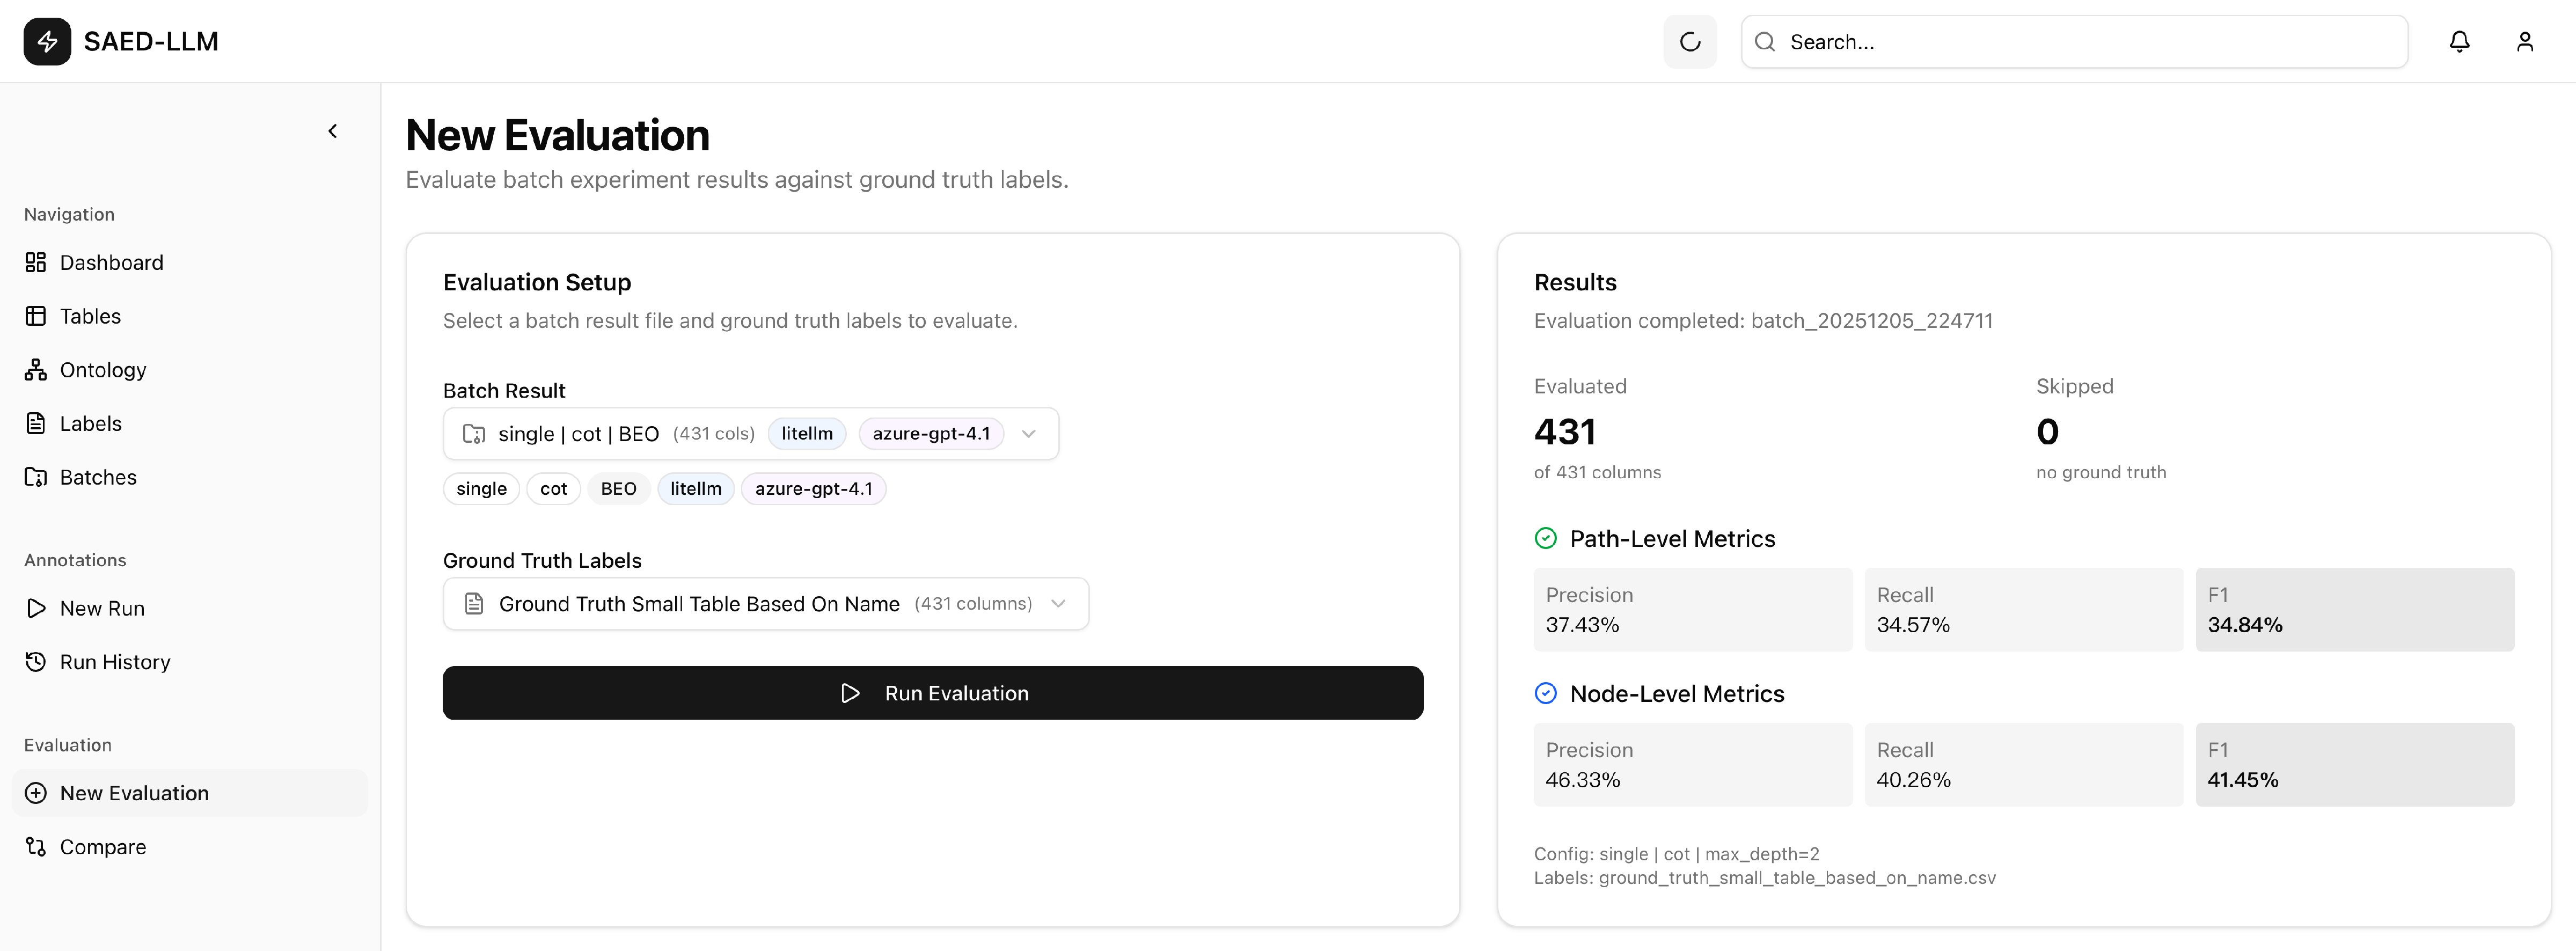
\includegraphics[width=\textwidth]{graphics/canvas/appendix_evaluation.pdf}
    \caption{Evaluation results view displaying annotation accuracy metrics.}
    \label{fig:webui-evaluation}
\end{figure}

\begin{figure}[htbp]
    \centering
    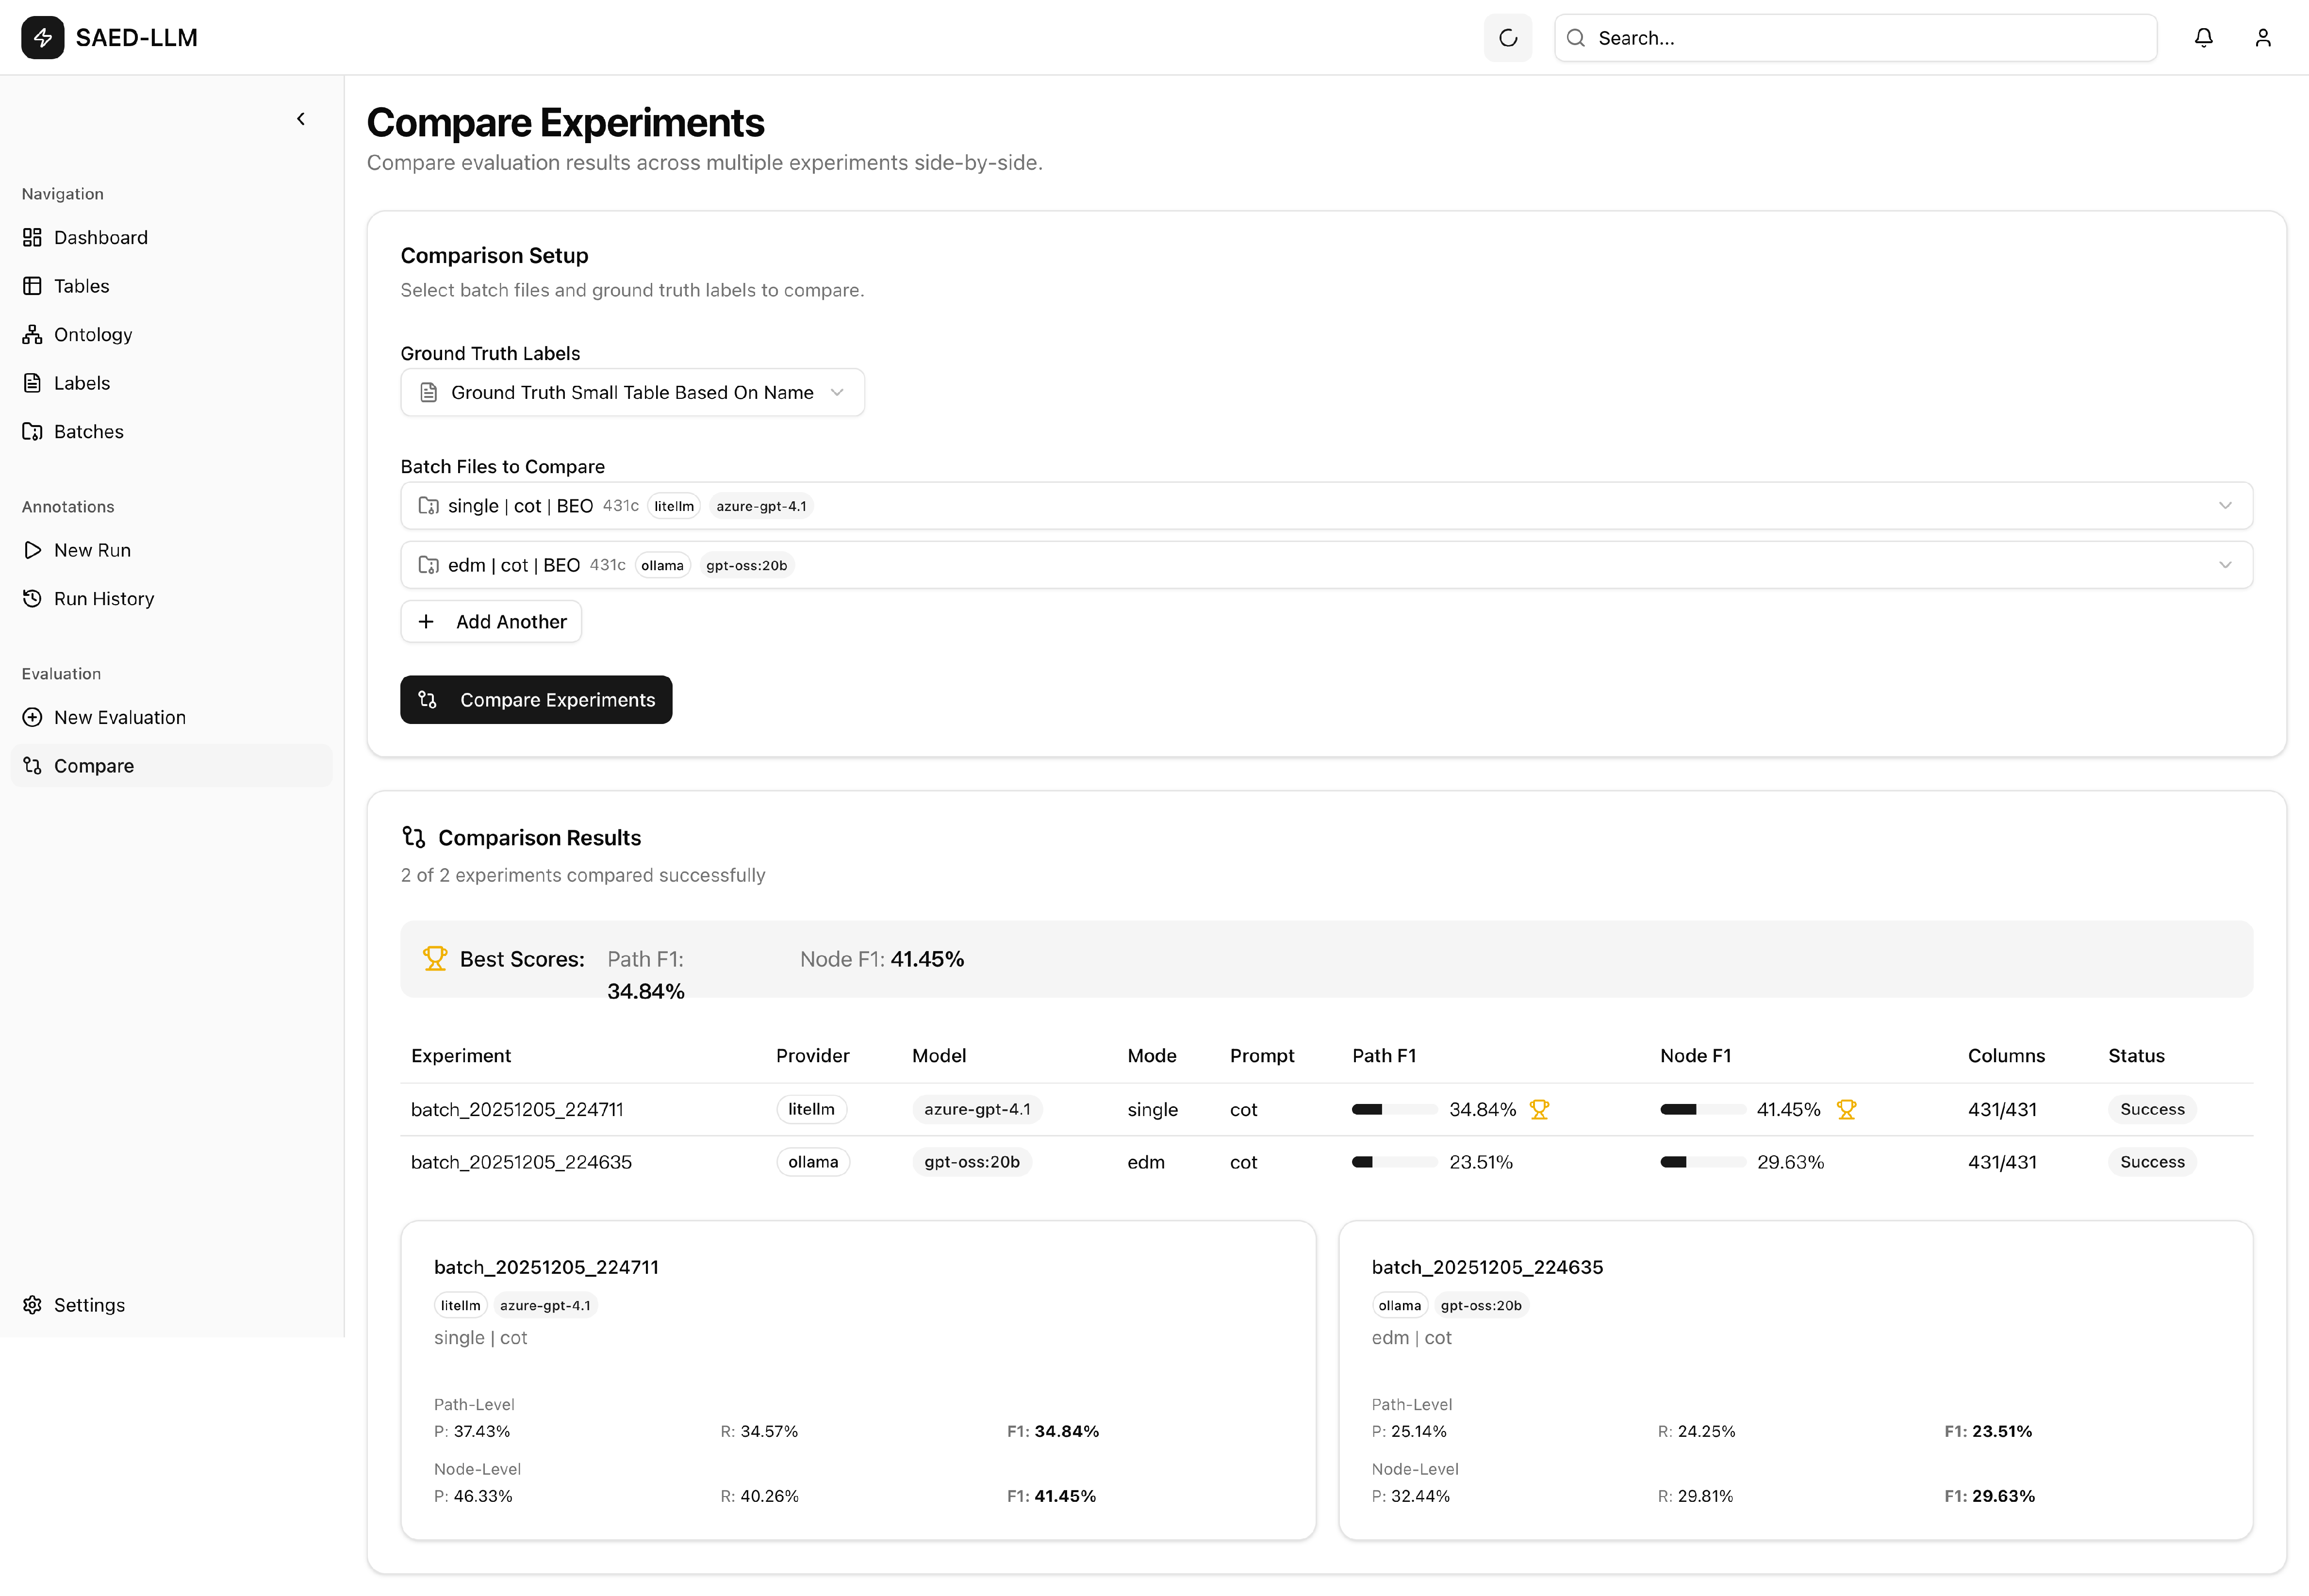
\includegraphics[width=\textwidth]{graphics/canvas/appendix_evaluation_compare.pdf}
    \caption{Evaluation comparison view for analyzing results across different experimental configurations.}
    \label{fig:webui-evaluation-compare}
\end{figure}
